\chapter[Well counters, radionuclide calibrators, survey meters]
        {Well counters, radionuclide calibrators and survey meters}

On many occasions, it is very handy or even essential to have
relatively simple devices to detect or quantify ionizing
radiation. Three important applications for such devices are:
\begin{itemize}
  \item To determine the amount of radioactivity in a syringe, so that
        one can adjust and/or verify how much activity is going to be
        administered to the patient.
  \item To determine the amount of radioactivity in a sample
        (usually blood samples) taken from the patient. The problem
        is the same as the former one, but the amount of radioactivity
        in a small sample is typically orders of magnitude less than
        the injected dose.
  \item To detect contaminations with radioactivity, e.g. due to
        accidents with a syringe or a phantom.
\end{itemize}
To use a PET or gamma camera for these tasks would obviously be
overkill (no imaging required), impractical (they are large and
expensive machines) and inefficient (for these tasks, relatively
simple systems with better sensitivity can be designed). Special
detectors have been designed for each of these tasks:
\begin{itemize}
  \item {\em the well counter}, for measuring small amounts of
        activity in small volumes,
  \item {\em the radionuclide calibrator} for measuring high amounts of
        activity in small volumes,
  \item {\em the survey meter} for finding radioactivity in places
        where there should be none.
\end{itemize}

\section{Well counter}
%%%%%%%%%%%%%%%%%%%%%
\begin{figure}[tb]
\centering
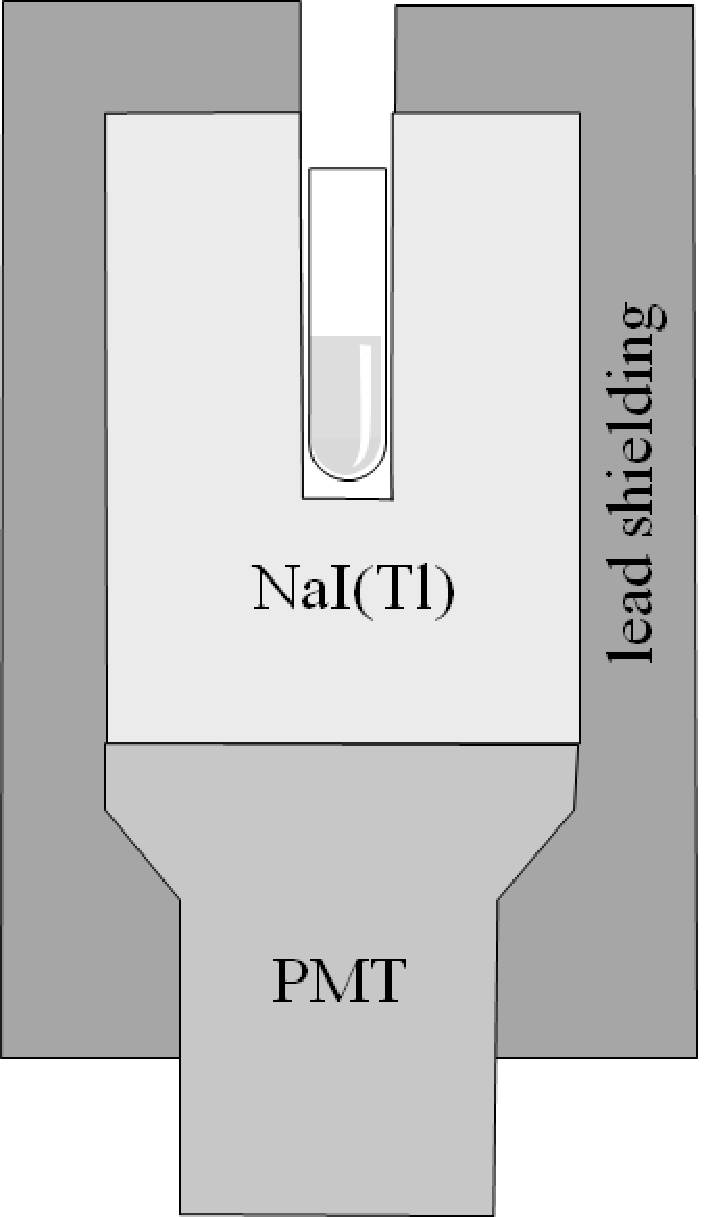
\includegraphics[width=0.3\textwidth]{figs/fig_wellcounter.pdf}
\caption{\label{fig:wellcounter} \emph{Diagram of a well counter, showing a
    test tube inside the well.}}
\end{figure}
The well counter consists of a scintillator crystal, typically
NaI(Tl), a PMT, lead shielding and electronics to control the PMT and
the user interface. The crystal has a cavity (the well), in which a
test tube (or any other small object) with a radioactive substance can
be put. As illustrated in fig. \ref{fig:wellcounter}, the radioactive
substance is almost completely surrounded by the scintillator
crystal. This gives the well counter an extremely high sensitivity,
enabling it to detect minute quantities of radioactivity. The well
counter detects individual photons, and similar to a gamma camera, it
can estimate the energy of the detected photon with an energy
resolution of about 10\%.

The crystal is usually several centimeters thick to further improve
the detection efficiency. The efficiency decreases (non-linearly) with
increasing energy, because photons with higher energy have a higher
probability of traveling through the crystal without interaction. The
effect of the crystal thickness can be taken into account by
calibrating the well counter, which is done by the vendor.
%
\begin{figure}[tb]
  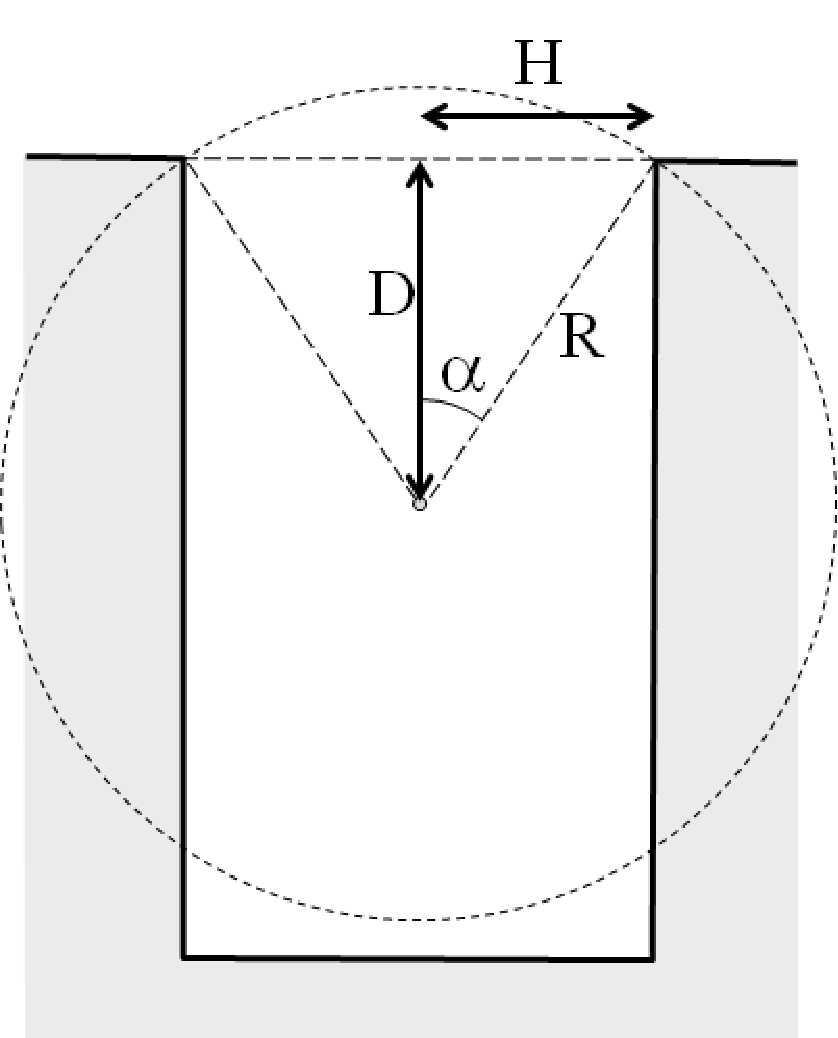
\includegraphics[width=0.35\textwidth]{figs/fig_wellcountersens.pdf}
  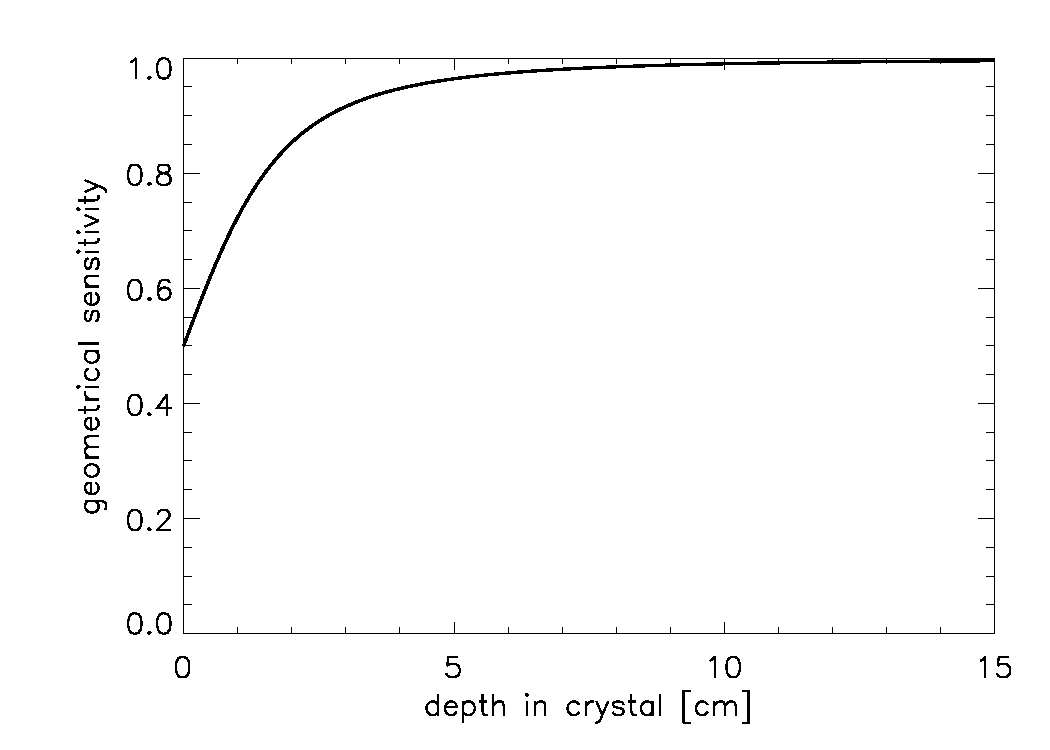
\includegraphics[width=0.61\textwidth]{figs/fig_wellcounter2.pdf}
\caption{\label{fig:wellcountersens} \emph{Left: diagram of a well counter, showing a
    test tube inside the well. Right: the geometrical sensitivity of
    the well counter to activity inside the tube, as a function of the
    depth inside the crystal ($H$ = 2 cm).}}
\end{figure}

One problem of the well counter is that its sensitivity varies with
the position of the source inside the crystal: the deeper a point
source is positioned inside the crystal, the smaller the chance that
its photons will escape through the entrance of the cavity. A simple
approximate calculation illustrates the effect. Suppose that the
radius of the cylindrical cavity is $H$ and that a point source is
positioned centrally in the hole at a depth $D$. As illustrated in
fig.\ \ref{fig:wellcountersens}, we have to compute the solid angle of
the entrance, as seen from the point source, to obtain the chance that
a photon escapes. A similar computation was done near equation
\eqref{eq:collim:fwhm}, but this time, we cannot ignore the curvature
of the sphere surface, because the entrance hole is fairly large:
\begin{equation}
 \mbox{escape-chance}(D)
  = \frac{1}{4\pi R^2}\int_0^\alpha 2\pi H'(\alpha') \; R d\alpha'
\end{equation}
where the value of $H'$ in the integral goes from $H'(0) = 0$ to
$H'(\alpha) = H$. A particular value of $\alpha'$ defines a circular
line on the sphere, and a small increment $d \alpha'$ turns the line
into a small strip with thickness $R d \alpha'$.
%
Substituting $H'(\alpha') = R \sin(\alpha'))$ one
obtains:
\begin{align}
  \mbox{escape-chance}(D)
 &= \frac{1}{4\pi R^2}\int_0^\alpha 2\pi R^2 \sin(\alpha') d\alpha' \nonumber\\
 &=  \frac{1}{2} \left. (- \cos(\alpha')) \right|_0^\alpha \nonumber\\
 &=  \frac{1}{2} (1 - \cos(\alpha)) 
     \;\; = \;\; \frac{1}{2}\left(1 - \frac{D}{\sqrt{D^2 + H^2}}\right)
     \label{eq:wellcounter}
\end{align}
And the chance that the photon will be detected equals
\begin{equation}
  \mbox{sensitivity}(D) = 1 - \mbox{escape-chance}(D) = \frac{1}{2}\left(1 + \frac{D}{\sqrt{D^2 + H^2}}\right) \ . 
  \label{eq:wellcountersens}
\end{equation}
We find that for $D = 0$, the sensitivity is 0.5, which makes sense,
because all photons going up will escape and all photons going down
will hit the crystal. For $D$ going to $\infty$, the sensitivity goes
to unity. Note that the equation also holds for negative $D$, which
means putting $D$ above the crystal. That makes the sensitivity
smaller than 0.5, and for $D = -\infty$, the sensitivity becomes zero.
A plot of the sensitivity as a function of the depth $D$ is also shown
in figure \ref{fig:wellcountersens}, for $H$ = 2 cm, i.e. a cylinder
diameter of 4 cm. This figure clearly shows that the sensitivity
variations are not negligible. One should obviously put objects as
deep as possible inside the crystal. Suppose we have two identical
test tubes, both with exactly the same amount of activity, but
dissolved in different amounts of water. If we measure the test tubes
one after the other with a well counter, putting each tube in exactly
the same position, the tube with less water will produce more counts!

Expression (\ref{eq:wellcountersens}) is approximate in an optimistic
way, because it ignores (amongst other effects) the possibility of a
photon traveling through the crystal without any interaction.
Although the well counter is well shielded, it not impossible that
there would be other sources of radioactivity in the vicinity of the
device, which could contribute a bit of radiation during the
measurement. Even a very small amount of background radiation could
influence the measurement, in particular if samples with very low
activity are being measured. For that reason, the well counter can do
a background measurement (simply a measurement without a source in the
detector), and subtract the recorded value from subsequent
measurements. Of course, if there would be a significant background
contribution, it would usually be much better to remove or shield it
than to leave it there and correct for it.

\section{Radionuclide calibrator}
%%%%%%%%%%%%%%%%%%%%%%%%%
Because the radionuclide calibrator is a gas filled detector, a small introduction
to gas filled detectors is given first.

\subsection{Gas filled detectors}
%--------------------------------
A gas filled detector consists of an anode and a cathode with a gas
between them. When a photon or particle travels through the gas, it
will ionize some of the atoms in the gas. If there would be no voltage
difference between the anode and the cathode, the electrons and ions
would recombine. But with a non-zero voltage, the electrons and
positive ions travel to the anode and cathode respectively, creating
a small current. If enough atoms are ionized, that current can be
measured. A cartoon drawing is shown in figure \ref{fig:gasdetector}.

If the voltage between the cathode and the anode is low, the electrons
and ions travel slowly, and have still time to recombine into
neutral atoms. As a result, only a fraction of them will reach the
electrodes and contribute to a current between anode and cathode.
That fraction increases with
increasing voltage, until it becomes unity (i.e. all ionizations
contribute to the current). Further increases in the voltage have
little effect on the measured current. This first plateau in the
amplitude vs voltage curve (fig \ref{fig:gasdetector}) is the
region where {\em ionization chambers} are typically operated. In this mode,
the output is proportional to the total number of ionizations, which in
turn is proportional to the energy of the particles. A single particle
does not produce a measurable current, but if many particles travel
through the ionization chamber, they create a measurable current which
is proportional to the total energy deposited in the gas per unit of time.
%
\begin{figure}[thb]
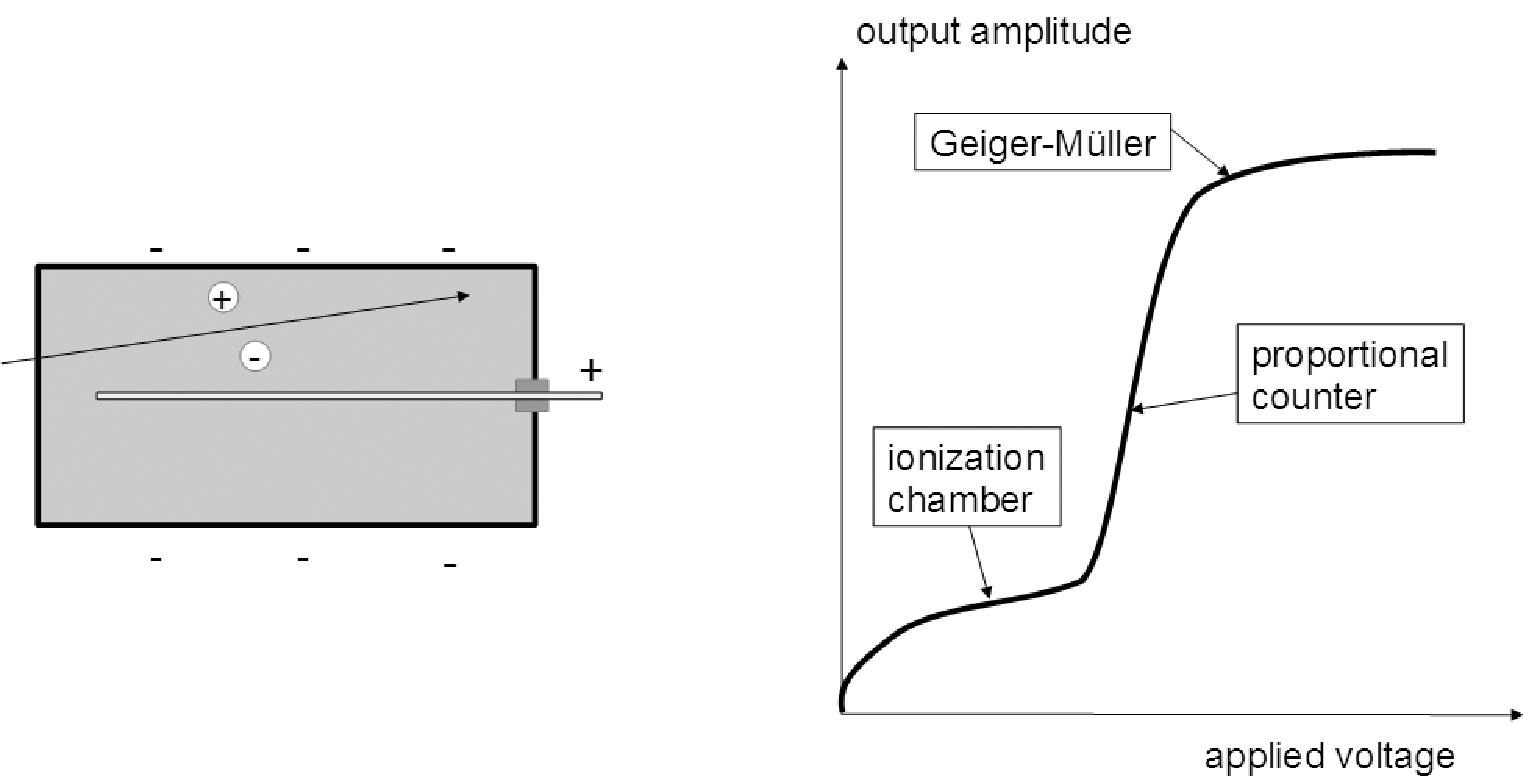
\includegraphics[width=0.8\textwidth]{figs/fig_gasdetector.pdf}
\caption{\label{fig:gasdetector} \emph{The gas detector.
Left: the detector consists of a box containing a gas. In this drawing,
the anode is a central wire, the cathode is the surrounding box. A photon
or particle traveling through the gas produces ionizations, which produce
a current between anode and cathode. Right: the current created by
a particle depends on the applied voltage.}}
\end{figure}

With increasing voltage, the speed of the electrons pulled towards the
anode increases. If that speed is sufficiently high, the electrons
have enough energy to ionize the gas atoms too. This avalanche
effect increases the number of ionizations, resulting in a magnification
of the measured current. This is the region where proportional
counters are operated. As schematically illustrated in fig
\ref{fig:gasdetector}, the amplification increases with the voltage.
In this mode, a single particle can create a measurable current, and
that current is proportional to the energy deposited by that particle 
in the gas.

With a still higher voltage, the avalanche effect is so high that
a maximum effect is reached, and the output becomes independent of the
energy deposited by the traversing particle. The reason is that the
electrons hit the anode with such a high energy that UV photons are
emitted. Some of those UV photons travel through the gas and liberate
even more electrons. In this mode, the gas detector
can  be used as a Geiger-M\"uller counter.
%
\footnote{Special tricks must actually be used
to make sure that the avalanche dies out after a while, 
the avalanche must be quenched. A common approach is to
use "quenching gases", which happen to have the right features
to avoid the excessive positive feedback that would maintain the
ionization avalanche.}
%
The Geiger-M\"uller counter detects individual particles, but its
output is independent of the energy deposited by the particle.


\subsection{Radionuclide calibrator}
%---------------------------
A radionuclide calibrator looks similar to a well counter, it also has a small
cylindrical hole surrounded by the detector. But instead of a crystal
with PMT, an ionisation chamber is used.
%
The output of the detector is proportional to the total number of
ionized gas atoms, which in turn is proportional to the energy
deposited in the gas, and therefore also proportional to the activity
put in the detector gap. The detector measures the contribution of
many photons simultaneously, and therefore it obtains no information
about the energy of individual photons. This lack of energy
discrimination is a drawback, but the capability of dealing with many
simultaneous incident photons (or other particles) makes this detector
useful for the measurement of high activities (which would saturate
photon counting devices, see section \ref{sec:deadtime}).

Ionisation chambers often use air, but for radionuclide calibrators, typically
pressurised Argon is used. The high pressure in the chamber reduces
the sensitivity to the atmospheric pressure. In addition, the high
pressure (more atoms) and the higher attenuation of Ar improve the
sensitivity of the detector. Radionuclide calibrators designed for higher
activities (up to $\pm$ 20 Ci or $\pm$ 750 GBq) use typically a
pressure of around 5 bar. These radionuclide calibrators are more likely to be
found at PET sites, where higher activities can be used because of the
short half lifes of most PET isotopes. For quantifying lower
activities (up to $\pm$ 5 Ci or $\pm$ 200 GBq), radionuclide calibrators with
a higher pressure ($\pm$ 12 bar) are used, because a higher pressure
improves the stability for low activity counting.

Since the geometry of the radionuclide calibrator is similar to that
of the well counter, it suffers from the same position dependent
response illustrated in fig.\ \ref{eq:wellcountersens}. But in
contrast to the well counter, the response of the radionuclide
calibrator is also heavily dependent upon the energy of the photons
emitted by the isotope.  The photons have to reach the gas, and to do
so, they must travel through the water in the test tube, through the
wall of the test tube and through the wall of the radionuclide
calibrator. Then, they have to interact with the gas to produce
ionisations. The probability of interactions (attenuation) decreases
with increasing energy. Finally, in every interaction, a few tens of
eV are transferred, so the higher the energy of the photon, the more
ionisations that same photon could produce. These three effects are
illustrated in figure \ref{fig:dosecalib}. The figure also shows their
product, which has a sharp local maximum at low energies, and
increases with increasing energy. This is only a rough approximation,
the actual curve for a particular radionuclide calibrator depends on
many things and it is safer (and much easier) to measure it than to
compute it. Knowing the emissions of a particular isotope, and the
sensitivity of the radionuclide calibrator for each of those
emissions, one can deduce the activity of the isotope from the
radionuclide calibrator measurement. A well calibrated radionuclide
calibrator will do this automatically for you, you only have to tell
it which isotope you are measuring, typically by selecting it from a
menu.

The high sensitivity at low energies can be problematic for isotopes
such as $^{123}$I and $^{111}$In, which emit a fairly large amount of
low energy photons (see table \ref{tab:dosiscalib}). The problem is
that these low energy photons are easily attenuated by a little bit of
water or a small amount of glass, and therefore, the dosis calibrator
would give very different responses when measuring the same activity
in different test tubes. The reproducibility improves dramatically
when these photons are eliminated by adding a bit of attenuating
material, such as a ``Cu-filter''. This filter is basically a copper
recipient with a very thin wall (half a mm or less), which has very
high attenuation for low energies, but only moderate attenuation for
higher energies. This is illustrated in the right panel of fig.\
\ref{fig:dosecalib}.

\begin{table}
\centering
\caption{Emissions of $^{123}$I and $^{111}$In.}
\label{tab:dosiscalib}
\begin{tabular}{|c|c|c|c|}
\hline
 Energy [keV]  & Iodine-123 emissions &    Energy & Indium-111 emissions  \\
    159    &      83.5\% & 172 & 90\% \\
           &             & 247 & 94\% \\
    27     &   71 \%     & 23  & 70\% \\
    31     &   15 \%     & 26  & 14\% \\
\hline
\hline
\end{tabular}
\end{table}

\begin{figure}[tb]
\hspace{-4mm}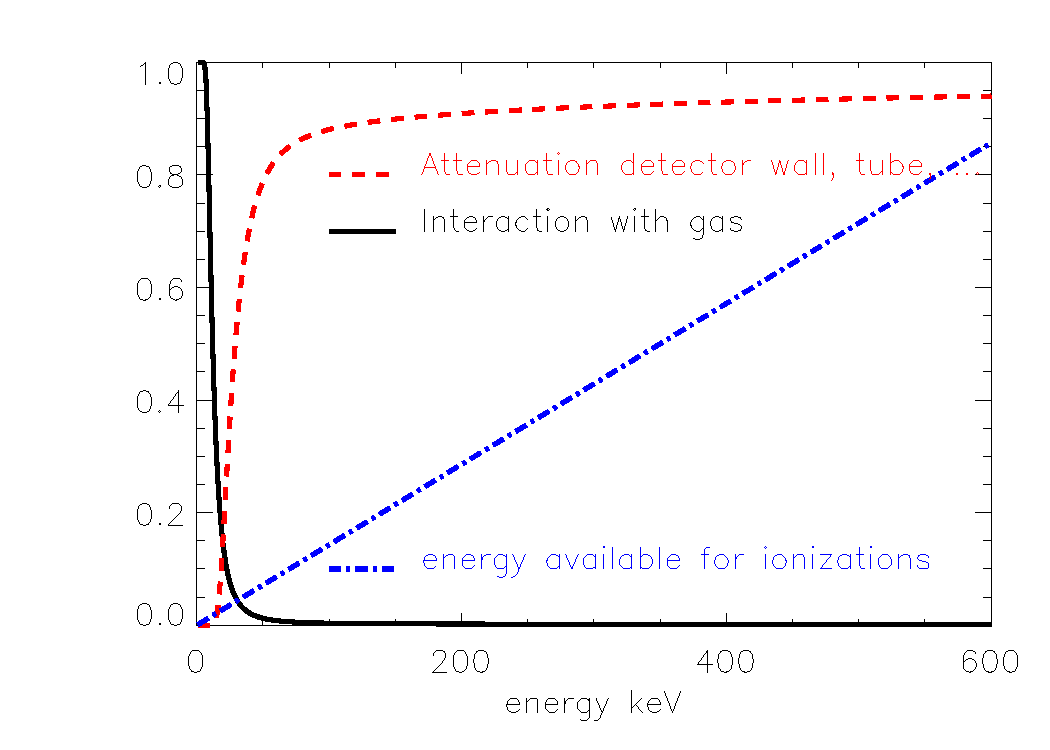
\includegraphics[width=0.53\textwidth]{figs/fig_dosecalib1.pdf}
        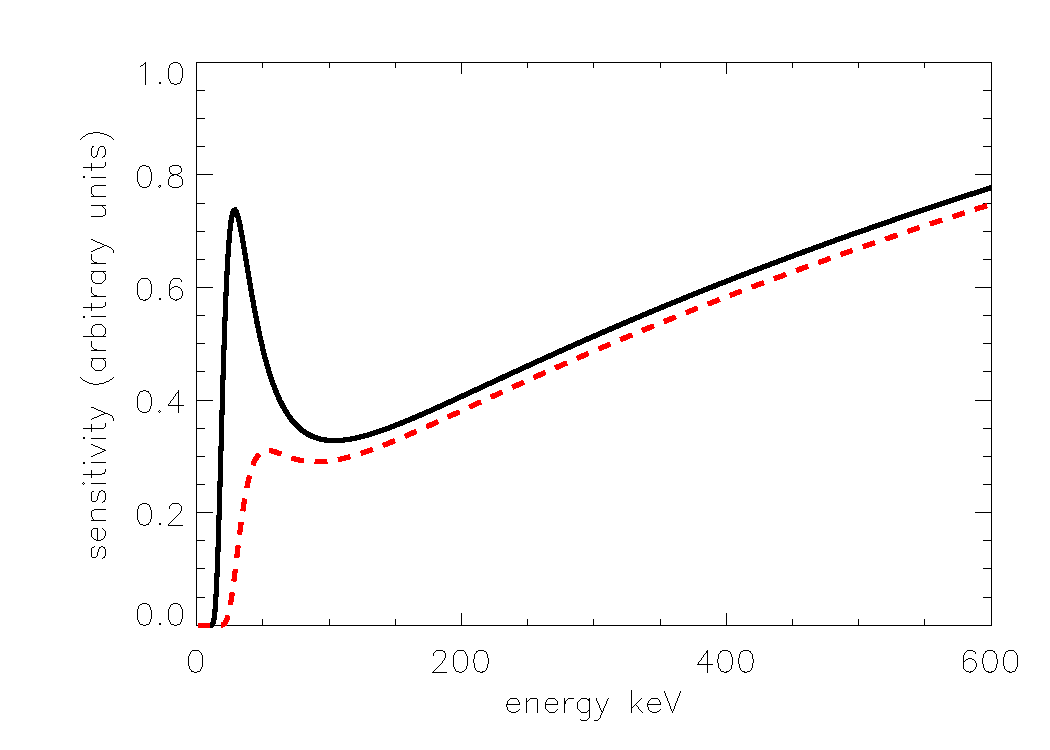
\includegraphics[width=0.53\textwidth]{figs/fig_dosecalib2.pdf}
\caption{\label{fig:dosecalib} \emph{Left: loss of photons due to
    attenuation in the test tube, detector wall etc., probability of
    interaction of the photons with the gas and the number of
    ionisations that could be produced with the energy of the photon
    (in arbitrary units), all as a function of the photon
    energy. Right: the combination of these three effects yields the
    sensitivity of the radionuclide calibrator as a function of the photon
    energy (solid line). The dashed line shows the sensitivity when
    the sample is surrounded by an additional Cu-filter of 0.2 mm thick.}}
\end{figure}

Just like the well counter, the dosis calibrator can measure the
background contribution and correct for it during measurements of
radioactive sources.

Radionuclide calibrators are designed to be very accurate, but to fully
exploit that accuracy, they should be used with care (e.g. using
Cu-filters when needed, position the syringe correctly et), and their
performance should be monitored with a rigorous quality control
procedure.

An important quality control test is to verify the linearity of the
radionuclide calibrator over the entire range of activities that is
supported, from 1 MBq to about 400 GBq.

\section{Survey meter}
%%%%%%%%%%%%%%%%%%%%%%
Survey meters are small hand held, battery powered devices, usually
containing a gas detector, i.e. an unshielded ionization chamber,
proportional counter or Geiger-M\"uller counter. Survey meters based
on ionization chambers basically measure the energy deposited in a
particular mass of air, i.e. the {\em air Kerma}, where ``Kerma''
stands for ``kinetic energy released in media''. Air Kerma is the
amount of energy per unit mass released in air, and has units of
Gy. The output of such a dosimeter would then typically be expressed
in microGy/hr or similar unit. Since the attenuation per gram air is
similar to the attenuation per gram tissue, air Kerma provides a
reasonable estimate of the absorbed dose in human tissues produced by
the radiation, the conversion factor is about 1.1, so
\begin{equation}
  \mbox{(absorbed dose in water or tissue)} \; \simeq \; 1.1 \; \times \;
    \mbox{(air Kerma)}.
\end{equation}

Other types of survey meters use a Geiger-M\"uller counter.
Often the device has a microphone and makes a
clicking sound for every detected particle. The Geiger-M\"uller
counter counts the incoming photons (or other particles), but it does
not measure its energy.

Finally, still other survey meters contain a scintillation crystal
with photomultiplier. These are also called ``contamination
monitors'', because they can be used to measure the spectrum of the
activity, to find out which tracer has caused the contamination.  This
is important information: a contamination with a long lived tracer is
obviously a more serious problem than with a short lived tracer.

Most survey meters can usually measure both photons and beta-particles
(electrons and positrons). Remember that to measure contamination with
beta-particles, the survey meter must be hold at small distance, because
in contrast to x-rays or gamma rays,
beta-particles have non-negigible attenuation in air.